% !TEX TS-program = lualatex
% !TEX encoding = UTF-8

\documentclass[twoside]{book}

%%%%%%%%%%%%%%% STANDARD PACKAGES %%%%%%%%%%%%%%%

\usepackage[paperwidth=148mm, paperheight=210mm]{geometry}

\usepackage{fontspec}
\usepackage[medievallatin, french]{babel}
\usepackage{fancyhdr}
\usepackage{paracol}
\usepackage{expl3}
\usepackage{needspace}
\usepackage{etoolbox}
\usepackage{tableof}
\usepackage{setspace}
\usepackage{alltt}
\usepackage{titlesec}
\usepackage{xcolor}
\usepackage{xstring}
\usepackage{enumitem}
\usepackage{hyperref}
\usepackage{refcount}
\usepackage{graphicx}

%%%%%%%%%%%%%%% GEOMETRY %%%%%%%%%%%%%%%

%% This should mimic the layout of the recent Solesmes books.
\geometry{
inner=15mm,
outer=10mm,
top=15mm,
bottom=15mm,
headsep=3mm,
}

%% General scale of all graphical elements.
%% Values different from 1 are largely untested.
%% Used in those commands (e.g. everything FontSpec) that use a scale parameter.
\newcommand{\customscale}{1}

%% Provide the command \fpeval as a copy of the code-level \fp_eval:n.
%% \fpeval allows to evaluate floating point calculation for scaled parameters, e.g. \setSomeStretchFactor{\fpeval{0,6 * \customscale}}
\ExplSyntaxOn
\cs_new_eq:NN \fpeval \fp_eval:n
\ExplSyntaxOff

%% No indentation of paragraphs
\setlength{\parindent}{0mm}

%% We want to allow large inter-words space 
%% to avoid overfull boxes in two-columns rubrics.
\sloppy

%%%%%%%%%%%%%%% GREGORIO CONFIG %%%%%%%%%%%%%%%

\usepackage[autocompile]{gregoriotex}

%% disable NABC a the request of A. Guyard who will add SG neumes by hand
\gresetnabc{1}{invisible} 

%% text above lines shall be of color gregoriocolor
\grechangestyle{abovelinestext}{\color{gregoriocolor}\footnotesize}
%% fine-tuning of space beween the staff and the text above lines
\newcommand{\altraise}{-1mm} %% default is -0.1cm
\grechangedim{abovelinestextraise}{\altraise}{scalable}

%% fine-tuning of space between the staff and the lyrics
\newcommand{\textraise}{2.8ex} %% default is 3.48471 ex
\grechangedim{spacelinestext}{\textraise}{scalable}

%% fine-tuning of space between the initial and the annotations
\newcommand{\annraise}{0mm} %% default is -0.2mm
\grechangedim{annotationraise}{\annraise}{scalable}

%% \officepartannotation converts a letter (IHARPT) into the office part to be printed as annotation,
%% storing the result into \result.

\newcommand{\result}{}
\newcommand{\lookup}[3]{%
  \IfSubStr{#2}{#1}{ \renewcommand{\result}{#3} }{}%
}%
\newcommand{\officepartannotation}[1]{%
  \renewcommand{\result}{#1}%
  \lookup{#1}{T}{}%
  \lookup{#1}{H}{Hymn.}%
  \lookup{#1}{A}{Ant.}%
  \lookup{#1}{P}{}%
  \lookup{#1}{R}{Resp.}%
  \lookup{#1}{I}{Invit.}%
  \lookup{#1}{M}{Ad Magn.}%
  \lookup{#1}{B}{Ad Ben.}%
  \result%
}%

%% header capture setup for the mode
\gresetheadercapture{mode}{greannotation}{string}

%% the space above lines for scores with neumes
\newcommand{\neumespace}{10mm}

%% outputs a score with no initials or annotations
%% for 
\newcommand{\smallscore}[2][y]{
  \gresetinitiallines{0}
  \ifx y#1\grechangedim{spaceabovelines}{\neumespace}{scalable}\null \vspace*{0.8\neumespace}\fi
  \gregorioscore{partitions/#2}
  \ifx y#1\grechangedim{spaceabovelines}{0mm}{scalable}\fi
  \gresetinitiallines{1}
}

%% outputs a score with annotations. no initials if [n] is passed
\newcommand{\gscore}[4][y]{
  %% #1 (passed as option) : y = space above lines for neumes, n = no such space
  %% #2 : name of the score file, should be a code, e.g. Q4F4A3 or 1225N1R1
  %% #3 : type of the score
  %% #4 : if applicable, a number between 1 and 9 (rank of the ant./resp.) - else: empty
  
  %% this prevents orphans
  \needspace{4\baselineskip} 
  \greannotation{\officepartannotation{#3}#4}
  \ifx y#1\grechangedim{spaceabovelines}{\neumespace}{scalable}\null \vspace*{0.8\neumespace}\fi
  \gregorioscore{partitions/#2}
  \ifx y#1\grechangedim{spaceabovelines}{0mm}{scalable}\fi
}

%%%%%%%%%%%%%%% FONTS %%%%%%%%%%%%%%%

%%%%%%%%%%%%%%% Main font
\setmainfont[Ligatures=TeX, Scale=\customscale]{Charis SIL}
%\setmainfont[Ligatures=TeX, Scale=\customscale]{TeXGyreBonum-Regular}
\setstretch{\fpeval{1.05 * \customscale}}

%%%%%%%%%%%%%%% Score initials
%% \initialsize resizes the initials, with one argument (size in points)
\newcommand{\initialsize}[1]{
    \grechangestyle{initial}{\fontspec{Zallman}\fontsize{#1}{#1}\selectfont}
}
%% default initial size is 32 points
\newcommand{\defaultinitialsize}{32}
\initialsize{\defaultinitialsize}

%% spacing before and after initials to kern the Zallman Caps.
%% this should be changed if we move away from Zallman Caps.
\newcommand{\initialspace}[1]{
  \grechangedim{afterinitialshift}{#1}{scalable}
  \grechangedim{beforeinitialshift}{#1}{scalable}
}
%% default space before and after initials is 0cm.
\newcommand{\defaultinitialspace}{0.9mm}
\initialspace{\defaultinitialspace}

%%%%%%%%%%%%%%% Score annotations
\grechangestyle{annotation}{\small}

%%%%%%%%%%%%%%% GRAPHICAL ELEMENTS %%%%%%%%%%%%%%%

%% V/, R/, A/ and + signs for in-line use (\vv \rr \aa \cc) and in-score use (<sp>V/ R/ A/ +</sp>)
\newcommand{\specialcharhsep}{3mm} % space after invoking R/ or V/ or A/
\newcommand{\vv}{\textcolor{gregoriocolor}{\fontspec[Scale=\customscale]{Charis SIL}℣.\hspace{\specialcharhsep}}}
\newcommand{\rr}{\textcolor{gregoriocolor}{\fontspec[Scale=\customscale]{Charis SIL}℟.\hspace{\specialcharhsep}}}
\renewcommand{\aa}{\textcolor{gregoriocolor}{\fontspec[Scale=\customscale]{Charis SIL}\Abar.\hspace{\specialcharhsep}}}
\newcommand{\cc}{\textcolor{gregoriocolor}{\fontspec[Scale=\customscale]{FreeSerif}\symbol{"2720}~}}
\gresetspecial{V/}{\textcolor{gregoriocolor}{\fontspec[Scale=\customscale]{Charis SIL}℣.~}}
\gresetspecial{R/}{\textcolor{gregoriocolor}{\fontspec[Scale=\customscale]{Charis SIL}℟.~}}
\gresetspecial{A/}{\textcolor{gregoriocolor}{\fontspec[Scale=\customscale]{Charis SIL}\Abar.~}}
\gresetspecial{+}{\textcolor{gregoriocolor}{\fontspec[Scale=\customscale]{FreeSerif}†~}}
\gresetspecial{‡}{\textcolor{gregoriocolor}{\fontspec[Scale=\customscale]{FreeSerif}‡~}}
\gresetspecial{*}{\gresixstar}

%% Roman Numerals
\usepackage{modroman}
\newcommand{\Rnum}[1]{\nbRoman{#1}}
\newcommand{\rnum}[1]{\nbshortroman{#1}}

%% Macro to print versicles
\newcommand{\versiculus}[2]{\rr #1 \\ \vv #2}

\newcommand{\versiculustpall}[2]
	{\versiculus{#1 \rubric{(T.P.} Allelúja. \rubric{)}}{#2 \rubric{(T.P.} Allelúja. \rubric{)}}}

%% Macro to print rubrics
\newcommand{\rubric}[1]{\textcolor{gregoriocolor}{\emph{#1}}}

%% Macro to print alternative text (feminine) between red parentheses
\newcommand{\bracketed}[1]{{\textcolor{gregoriocolor}(}#1{\textcolor{gregoriocolor})}}

%% Macro to print the name of a score in normal characters inside a \rubric
\newcommand{\normaltext}[1]{{\normalfont\normalcolor #1}}
\newcommand{\scorename}[1]{\normaltext{\nameref{#1}}}

%% Macro to print the common rubric that signals the Te Deum
\newcommand{\tedeumrubric}{\rubric{Lectione ultima peracta Hymnus \normaltext{Te Deum} cantatur.}}

%% Macro to print translations
\newcommand{\trans}[1]{	\emph{#1}}

%% This defines the star character used for mediants in text
\newcommand{\psstar}{\gresixstar}

%% Custom separator
\newcommand{\customseparator}{\vfill{\centering \greseparator{2}{18}\par}\vfill}

%%%%%%%%%%%%%%% COLUMN MANAGEMENT %%%%%%%%%%%%%%%

\usepackage{multicol}
\usepackage{parcolumns}
\setlength\columnseprule{0.4pt}

%% Macros to print a psalm on two columns.
%% First, without title and incipitur

\newcommand{\psalmtext}[1]{
	\needspace{2\baselineskip}
	\vspace{\baselineskip}
	\begin{parcolumns}[rulebetween]{2}%
	\colchunk{%
		\vspace{-\baselineskip}
		\begin{itemize}[%
			label=\null, %
			leftmargin=0pt, %
			itemindent=3mm, %
			labelsep=0pt, %
			labelwidth=0pt, %
			rightmargin=0pt, %
			parsep=0pt, %
			topsep=0pt, %
			itemsep=0pt]%
		\input{psaumes/#1_la.tex}%
		\end{itemize}%
	}%
	\colchunk{%
		\vspace{-\baselineskip}
		\begin{itemize}[%
			label=\null, %
			leftmargin=0pt, %
			itemindent=3mm, %
			labelsep=0pt, %
			labelwidth=0pt, %
			rightmargin=0pt, %
			parsep=0pt, %
			topsep=0pt, %
			itemsep=0pt]%
		\input{psaumes/#1_fr.tex} %
		\end{itemize} %
	}%
	\end{parcolumns}
}

%% then, adding a title and incipitur
\newcommand{\psalmus}[2]{
	\needspace{4\baselineskip}
	\smalltitle{Psaume #1}
	\smallscore[n]{#2}
	\psalmtext{#1}
}

%% Macro to print lessons on two columns.

\newcommand{\lesson}[1]{
	
	~
	
	\begin{parcolumns}[rulebetween]{2}%
	\colchunk{%
		\input{lecons/#1_la.tex}%
	}%
	\colchunk{%
		\input{lecons/#1_fr.tex} %
	}%
	\end{parcolumns}
}

%%%%%%%%%%%%%%% HEADER STYLES %%%%%%%%%%%%%%%

\pagestyle{fancy}
\fancyhead{}
\fancyfoot{}
\renewcommand{\headrulewidth}{0pt}
\setlength{\headheight}{20pt}
\fancyhead[RO]{\small\rightmark\hspace{1cm}\thepage}
\fancyhead[LE]{\small\thepage\hspace{1cm}\leftmark}

\newcommand{\setheaders}[2]{
	\renewcommand{\rightmark}{{\sc#2}}
	\renewcommand{\leftmark}{{\sc#1}}
}
\setheaders{}{}

%%%%%%%%%%%%%%% TITLE STYLES %%%%%%%%%%%%%%%

%% Titles are centered and small-caps
\titleformat{\chapter}[block]{\Large\filcenter\sc}{}{}{}
\titleformat{\section}[block]{\large\filcenter\sc}{}{}{}
\titleformat{\subsection}[block]{\filcenter\sc}{}{}{}
\setcounter{secnumdepth}{0}
%% Fine-tuning of space around titles
\titlespacing*{\paragraph}{0pt}{1ex}{.6ex}


\newcommand{\officiumtitulum}[1]{
  \newpage
  \thispagestyle{empty}
  \setheaders{{\scshape #1}}{{\scshape #1}}
  \begin{center}
  {\scshape\LARGE #1}\par
  \end{center}
}

\newcommand{\smalltitle}[1]{
\needspace{5\baselineskip}
\vspace{\baselineskip}
 {\centering\scshape #1\par}
}

\newcommand{\nocturnumtitulum}[1]{
  %% needspace: should be barely more than the vertical space for the titles, rubrics excluded.
  %% this is to ensure that the page does not get cut after the title
  \needspace{10\baselineskip}
  \vspace{1cm}
  \begin{center}
  {\scshape\Large #1}\par
  \end{center}
}

\begin{document}

% ceci est pour conserver une numérotation ordinaire malgré paracol
\twosided[pb]

\begin{titlepage}
\centering\null

\vspace{1cm}

{\scshape\LARGE Officium Defunctorum}

\vspace{2cm}
{\scshape\Large juxta usum antiquiorem ritus romani}

\vspace{5cm}

{\scshape\LARGE L'Office des Morts}

\vspace{2cm}
{\scshape\Large selon l'usage ancien du rite romain}




\end{titlepage}

\thispagestyle{empty}

~

\vfill

\begin{center}
Nouvelles restitutions des antiennes et répons\\
Édition préparée par Matthias Bry, Dominique Crochu et Anne Guyard\\
Traduction des textes bibliques © AELF
\end{center}

\newpage
% tolérance infinie sur les sauts de lignes pour les colonnes étroites
\sloppy

\officiumtitulum{à Vêpres}

\rubric{L'office débute par la première antienne, sans aucune introduction. Il n'y a ni hymne ni capitule.}

\gscore{VA1}{A}{1}
~\\
\trans{\aa Je plairai au Seigneur dans la terre des vivants.}
\psalmus{114}{VP1}
\smallscore{VA1}

~\\

\gscore{VA2}{A}{2}
~\\
\trans{\aa Malheur à moi car mon exil s'est prolongé.}
~\\
\psalmus{119}{VP2}
\smallscore{VA2}

\gscore{VA3}{A}{3}
~\\
\trans{\aa Le Seigneur te garde de tout mal, que le Seigneur garde ton âme.}

\psalmus{120}{VP3}
\smallscore{VA3}

\gscore{VA4}{A}{4}
~\\
\trans{\aa Si Tu retiens les fautes, Seigneur, Seigneur, qui subsistera ?}
~\\
\psalmus{129}{VP4}
\smallscore{VA4}
\vspace{2mm}

\gscore{VA5}{A}{5}
~\\
\trans{\aa Ne méprise pas, Seigneur, les œuvres de Tes mains.}
~\\
\psalmus{137}{VP5}
\smallscore{VA5}

\newpage

\smalltitle{Versicule}
\smallscore[n]{OR_audivi}
\trans{\vv J'entendis une voix du ciel qui me disait : \\ \rr Bienheureux les morts qui meurent dans le Seigneur.}

\vspace{\baselineskip}

\gscore{VAM}{M}{}
\trans{\aa Tout ce que le Père Me donne viendra à Moi ; et celui qui vient à Moi, Je ne le jetterai pas dehors.}

\smalltitle{Cantique de Marie}
\smallscore[n]{VPM}
\psalmtext{m}
\smallscore{VAM}

\newpage

\smalltitle{Conclusion}

~

\rubric{Toute la conclusion de l'office se chante à genoux.\\Sauf la dernière, toutes les réponses se disent sur ce ton :}

\smallscore[n]{OR_tonusversus}
~\\
\begin{parcolumns}[rulebetween]{2}%
	\colchunk{%
		\vv Pater noster...\\
		\rubric{(en silence jusqu'à :)}\\
		\vv Et ne nos indúcas in tentatiónem: \\
		\rr Sed líbera nos a malo.
	}
	\colchunk{%
		\vv Notre Père...\\
		\vv Et ne nous laisse pas entrer en tentation.\\
		\rr Mais délivre-nous du mal.
	}
\end{parcolumns}

\rubric{Selon une ancienne coutume, on chantait ici le psaume 145 comme indiqué page~\pageref{ps145}. Aujourd'hui ce psaume est omis.}

\begin{parcolumns}[rulebetween]{2}%
	\colchunk{%
		\vv A porta ínferi.\\
		\rr Erue, Dómine, ánimam ejus \bracketed{ánimas eórum}.\\
		\vv Requiéscat in pace. \bracketed{Requiéscant in pace.}\\
		\rr Amen.\\
		\vv Dómine, exáudi oratiónem meam.\\
		\rr Et clamor meus ad te véniat.\\
		\vv Orémus.
	}
	\colchunk{%
		\vv De la puissance de l'enfer.\\
		\rr Délivre, Seigneur, son âme \bracketed{leurs âmes}.\\
		\vv Qu'il repose en paix. \bracketed{Qu'ils reposent en paix.}\\
		\rr Amen.\\
		\vv Seigneur, entends ma prière.\\
		\rr Et que mon cri parvienne jusqu'à Toi.\\
		\vv Prions.
	}
\end{parcolumns}

\rubric{On dit l'oraison qui correspond à l'occasion, pages suivantes, et on répond \normaltext{Amen.} Puis, on dit, toujours au pluriel :}

\begin{parcolumns}[rulebetween]{2}%
	\colchunk{%
		\vv Réquiem ætérnam dona eis, Dómine.\\
		\rr Et lux perpétua lúceat eis.
	}
	\colchunk{%
		\vv Seigneur, donne-leur le repos éternel.\\
		\rr Et fais luire pour eux la lumière sans déclin.
	}
\end{parcolumns}

\smallscore[n]{OR_requiescant}
~\\
\trans{\vv Qu'ils reposent en paix.\\ \rr Amen.}

\officiumtitulum{Oraisons}

{\centering \rubric{À dire à la fin des offices, en fonction de diverses circonstances.}\par}
\label{oraisons}

\smalltitle{devant le corps du défunt}

~

\begin{parcolumns}[rulebetween]{2}%
	\colchunk{%
Deus, cui próprium est miseréri semper et párcere, te súpplices exorámus pro ánima fámuli tui \bracketed{fámulæ tuæ} N., quam hódie de hoc sǽculo migráre jussísti : † ut non tradas eam in manus inimíci, neque obliviscáris in finem, sed júbeas eam a sanctis angelis súscipi, et ad pátriam paradísi perdúci ;~\psstar{} ut quia in te sperávit et credidit, non pœnas inférni sustíneat, sed gaúdia ætérna possidéat. Per Dóminum nostrum Jesum Christum, Fílium tuum : qui tecum vivit et regnat in unitáte Spíritus Sancti, Deus, per ómnia sǽcula sæculórum.\\
\rr Amen.
	}
	\colchunk{%
Dieu, à qui appartiennent la miséricorde et le pardon, nous T'adressons nos supplications en faveur de l'âme de Ton serviteur \bracketed{Ta servante} N., que Tu as aujourd'hui retirée de ce monde. Ne la livre pas au mains de l'ennemi, et ne l'ouble pas pour toujours ; mais ordonne à Tes anges de la recevoir et de la conduire au ciel, sa patrie. Fais que, après avoir cru et espéré en Toi, elle n'ait pas à souffrir les peines de l'enfer, mais qu'elle entre en possession des joies éternelles.
	}
\end{parcolumns}

\smalltitle{le jour des funérailles}

~

\begin{parcolumns}[rulebetween]{2}%
	\colchunk{%
Absólve, quǽsumus Dómine, ánimam fámuli tui \bracketed{fámulæ tuæ} N., ut defúnctus \bracketed{defúncta} sǽculo tibi vívat : † et quæ per fragilitátem carnis humána conversatióne commísit,~\psstar{} tu vénia misericordíssimæ pietátis abstérge. Per Dominum.
	}
	\colchunk{%
Délivre, Seigneur, nous T'en supplions, l'âme de Ton serviteur \bracketed{Ta servante}, afin que, ayant quitté ce monde, elle vive en Toi ; et les fautes que la fragilité de la chair lui a fait commettre durant cette vie, efface-les, par un effet de Ta miséricordieuse bonté.
	}
\end{parcolumns}
\newpage
\smalltitle{le troisième, septième, trentième jour après la mort}

~

\begin{parcolumns}[rulebetween]{2}%
	\colchunk{%
Quǽsumus Dómine, ut ánimæ fámuli tui \bracketed{fámulæ tuæ} N., cujus depositiónis diem tértium \rubric{\emph{(}vel} séptimum\rubric{, vel} trigésimum\rubric{\emph{)}} commemorámus,~† sanctórum atque electórum tuórum largíri dignéris consórtium ;~\psstar{} et rorem misericórdiæ tuæ perénnem infúndas. Per Dóminum.
	}
	\colchunk{%
Seigneur, daigne accorder à l'âme de Ton serviteur \bracketed{Ta servante} N., dont nous faisons mémoire en ce troisième \rubric{\emph{(}ou} septième \rubric{ou} trentième\rubric{\emph{)}} jour depuis sa mort, la société de Tes saints et de Tes élus ; répands aussi sur elle la rosée éternelle de Ta miséricorde.
	}
\end{parcolumns}

\smalltitle{le jour anniversaire de la mort}

~

\begin{parcolumns}[rulebetween]{2}%
	\colchunk{%
Deus indulgentiárum Dómine :~† da ánimæ fámuli tui N. \rubric{\emph{(}}fámulæ tuæ N.\rubric{, vel} animábus famulórumque tuárum\rubric{\emph{)}}, cujus \bracketed{quorum} anniversárium depositiónis diem commemorámus,~\psstar{} refrigérii sedem, quiétis beatitúdinem, et lúminis claritátem. Per Dóminum.
	}
	\colchunk{%
Seigneur, Dieu des miséricordes, accorde à l'âme de Ton serviteur \rubric{\emph{(}ou} de Ta servante\rubric{, ou} aux âmes de Tes serviteurs\rubric{\emph{)}}, dont nous célébrons aujourd'hui l'anniversaire, le lieu de rafraîchissement, le bonheur du repos et l'éclat de la lumière.
	}
\end{parcolumns}

\smalltitle{pour un Pape}

~

\begin{parcolumns}[rulebetween]{2}%
	\colchunk{%
Deus, qui inter summos sacerdótes fámulum tuum N. ineffábili tua dispositióne connumerári voluísti : † præsta, quǽsumus ; ut qui Unigéniti Fílii tui vices in terris gerébat,~\psstar{} sanctórum tuórum Pontíficum consórtio perpétuo aggregétur. Per eúmdem Dóminum.
	}
	\colchunk{%
Dieu, qui as voulu, par une providence ineffable, que Ton serviteur N. fût au nombre des Souverains Pontifes, fais, nous T'en prions, qu'ayant occupé sur la terre la place de Ton Fils unique, il partage à jamais le sort de Tes saints Pontifes dans le ciel.
	}
\end{parcolumns}

\smalltitle{pour un évêque}

~

\begin{parcolumns}[rulebetween]{2}%
	\colchunk{%
Deus, qui inter apostólicos sacerdótes fámulum tuum N. pontificáli fecísti dignitáte vigére :~† præsta, quǽsumus ;~\psstar{} ut eórum quoque perpétuo aggregétur consórtio. Per Dóminum.
	}
	\colchunk{%
Dieu, qui as élevé Ton serviteur N. à la dignité pontificale, en lui donnant part au sacerdoce des Apôtres, fais qu'il jouisse avec eux de la gloire éternelle.
	}
\end{parcolumns}

\smalltitle{pour un prêtre}

~

\begin{parcolumns}[rulebetween]{2}%
	\colchunk{%
Deus, qui inter apsotolícos sacerdótes fámulum tuum N. \bracketed{fámulos tuos N. et N.} sacerdotáli fecísti dignitáte vigére : † præsta, quǽsumus ;~\psstar{} ut eórum quoque perpétuo aggregétur \bracketed{aggregéntur} consórtio. Per Dóminum.

\rubric{Autre oraison pour un prêtre :}

Præsta, quǽsumus Dómine : † ut ánima fámuli tui N. sacredótis, quem in hoc sǽculo commorántem, sacris munéribus decorásti,~\psstar{} in celésti sede gloriósa semper exsúltet. Per Dóminum.
	}
	\colchunk{%
Dieu, qui as élevé Ton serviteur N. \bracketed{Tes serviteurs N. et N.} à la dignité sacerdotale, en lui \bracketed{leur} donnant part au sacerdoce des Apôtres, fais qu'il\bracketed{s} jouisse\bracketed{nt} avec eux de la gloire éternelle.

~

Accorde, nous t'en prions, Seigneur, que l'âme de Ton serviteur N., prêtre, qu'en ce monde Tu as honoré de la charge sacerdotale, se réjouisse éternellement dans le glorieux séjour céleste.
	}
\end{parcolumns}

\smalltitle{pour un homme}

~

\begin{parcolumns}[rulebetween]{2}%
	\colchunk{%
Inclína Dómine aurem tuam ad preces nostras, quibus misericórdiam tuam súpplices deprecámur :~† ut ánimam fámuli tui N., quam de hoc sǽculo migráre jussísti, in pacis ac lucis regióne constítuas,~\psstar{} et sanctórum tuórum júbeas esse consórtem. Per Dóminum.
	}
	\colchunk{%
Seigneur, prête l'oreille à nos prières, par lesquelles nous implorons humblement Ta miséricorde, afin que Tu introduises dans le séjour de la paix et de la lumière l'âme de Ton serviteur, que Tu as retirée de cette terre, et que Tu l'admettes dans la société de Tes saints.
	}
\end{parcolumns}

\smalltitle{pour une femme}

~

\begin{parcolumns}[rulebetween]{2}%
	\colchunk{%
Quǽsumus Dómine, pro tua pietáte miserére ánimæ fámulæ tuæ N. :~† et a contágiis mortalitátis exútam,~\psstar{} in ætérnæ salvatiónis partem restítue. Per Dóminum.
	}
	\colchunk{%
Seigneur, dans Ta bonté, aie pitié de l'âme de Ta servante N. : maintenant qu'elle est délivrée des tentations de cette vie mortelle, daigne l'établir dans l'héritage du salut éternel.
	}
\end{parcolumns}
\newpage
\smalltitle{pour un ou des frères, amis et bienfaiteurs}

~

\begin{parcolumns}[rulebetween]{2}%
	\colchunk{%
Deus, véniæ largítor et humánæ salútis amátor :~† quǽsumus cleméntiam tuam ; ut nostræ congregatiónis fratres, propínquos et benefactóres qui ex hoc sǽculo transiérunt,~\psstar{} beáta María semper Vírgine intercedénte cum ómnibus sanctis tuis, ad perpétuæ beatitúdinis consórtium perveníre concédas. Per Dóminum.
	}
	\colchunk{%
Dieu, qui accordes le pardon et qui veux le salut de l'homme, nous implorons Ta clémence : grâce à l'intercession de la bienheureuse Marie toujours Vierge, et de tous Tes saints, fais parvenir les âmes de nos frères, amis et bienfaiteurs qui ont quitté ce monde, à la participation de la béatitude éternelle.
	}
\end{parcolumns}
	
\smalltitle{pour un père et une mère}

~

\begin{parcolumns}[rulebetween]{2}%
	\colchunk{%
Deus, qui nos patrem et matrem honoráre præcepísti ;~† miserére cleménter animábus paréntum nostrórum, eorúmque peccáta dimítte :~\psstar{} nosque eos in ætérnæ claritátis gáudio fac vídere. Per Dóminum.
	}
	\colchunk{%
Dieu, qui nous as commandé d'honorer notre père et notre mère, aie pitié, dans Ta clémence, des âmes de nos parents, et pardonne leurs péchés. Accorde-nous de les revoir un jour dans la joie de la gloire éternelle.
	}
\end{parcolumns}
	
\smalltitle{pour plusieurs défunts}

~

\begin{parcolumns}[rulebetween]{2}%
	\colchunk{%
Deus, cui próprium est miseréri semper et párcere :~† propitiáre animábus famulórum famularúmque tuárum, et ómnia eórum peccáta dimítte ;~\psstar{} ut mortalitátis vínculis absolútæ, transíre mereántur ad vitam. Per Dóminum. 

~

\rubric{Autre oraison pour plusieurs défunts :}

Animábus, quǽsumus Dómine, famulórum famularúmque tuárum misericórdiam concéde perpétuam :~† ut eis profíciat in ætérnum,~\psstar{} quod in te speravérunt et credidérunt. Per Dóminum.
	}
	\colchunk{%
Dieu, à qui appartiennent la miséricorde et le pardon, jette un regard de bienveillance sur les âmes de Tes serviteurs et de Tes servantes, et pardonne tous leurs péchés : afin que, dégagées des liens de cette vie mortelle, elles puissent entrer dans la vie éternelle.

~

Accorde, nous T'en prions, Seigneur, la miséricorde éternelle aux âmes de Tes serviteurs et de Tes servantes, afin que leur espérance et leur foi en Toi leur soient profitables pour l'éternité.
	}
\end{parcolumns}

\vfill

\pagebreak

\smalltitle{à l'office des défunts pendant l'année}

~

\rubric{On peut dire seulement la troisième oraison \normaltext{Fidélium Deus ómnium}, ou la faire précéder des deux autres, selon une coutume ancienne, ces trois oraisons étant groupées sous la même conclusion.}

~

\begin{parcolumns}[rulebetween]{2}%
	\colchunk{%
Deus, qui inter apostólicos sacerdótes fámulos tuos pontificáli seu sacerdotáli fecísti dignitáte vigére :~† præsta, quǽsumus ;~\psstar{} ut eórum quoque perpétuo aggregétur consórtio.

~

Deus, véniæ largítor et humánæ salútis amátor :~† quǽsumus cleméntiam tuam ; ut nostræ congregatiónis fratres, propínquos et benefactóres qui ex hoc sǽculo transiérunt,~\psstar{} beáta María semper Vírgine intercedénte cum ómnibus sanctis tuis, ad perpétuæ beatitúdinis consórtium perveníre concédas.

~

Fidélium Deus ómnium cónditor et redémptor, animábus famulórum famularúmque tuárum remissiónem cunctórum tríbue peccatórum :~† ut indulgéntiam, quam semper optavérunt,~\psstar{} piis supplicatiónibus consequántur. Qui vivis et regnas cum Deo Patre, in unitáte Spíritus Sancti, Deus, per ómnia sǽcula sæculórum.
	}
	\colchunk{%
Dieu, qui as élevé Tes serviteurs aux dignités pontificale et sacerdotale, en leur donnant part au sacerdoce des Apôtres, fais qu'ils jouissent avec eux de la gloire éternelle.
	
~\\~

Dieu, qui accordes le pardon et qui veux le salut de l'homme, nous implorons Ta clémence : grâce à l'intercession de la bienheureuse Marie toujours Vierge, et de tous Tes saints, fais parvenir les âmes de nos frères, amis et bienfaiteurs qui ont quitté ce monde, à la participation de la béatitude éternelle.

~

Dieu, créateur et rédempteur de tous les fidèles, accorde aux âmes de Tes serviteurs et de Tes servantes, la rémission de tous leurs péchés afin que le pardon qu'ils ont toujours désiré leur soit obtenu par ces pieuses supplications. Toi qui vis et règnes avec le Père dans l'unité du Saint-Esprit, Dieu, pour les siècles des siècles.

	}
\end{parcolumns}

\customseparator{}

\officiumtitulum{à Matines}

\rubric{L'office débute par l'invitatoire, sans aucune introduction. Il n'y a pas d'hymne.  Les leçons sont chantées sans bénédiction ni absolution. On chante trois nocturnes le jour de la mort d'un défunt, le jour de sa sépulture, les troisième, septième, trentième jours après sa mort, et le jour anniversaire, et en toute autre occasion légitime. On chante un seul nocturne les autres jours, comme précisé ci-dessous.}

\smalltitle{Invitatoire}

\gscore[n]{MI}{I}{}

\nocturnumtitulum{Premier Nocturne}
\rubric{Si l'on chante un seul nocturne, ce nocturne se chante les dimanche, lundi et jeudi.}

\gscore{MA1}{A}{1}
~\\
\trans{\aa Redresse, Seigneur mon Dieu, Ton chemin devant moi.}
\psalmus{5}{MP1}

\begin{itemize}[%
			label=\null, %
			leftmargin=0pt, %
			itemindent=3mm, %
			labelsep=0pt, %
			labelwidth=0pt, %
			rightmargin=0pt, %
			parsep=0pt, %
			topsep=0pt, %
			itemsep=0pt]%
\item Dómine, ut scuto bonæ volun\textbf{tá}tis \textbf{tu}æ~\psstar{} \textbf{co}ro\textbf{nás}ti nos.
\item Réqui\textbf{em} æ\textbf{tér}nam~\psstar{} dona \textbf{e}is, \textbf{Dó}mine.
\item Et \textbf{lux} per\textbf{pé}tua~\psstar{} \textbf{lú}ceat \textbf{e}is.
\end{itemize}%
\newpage
\smallscore{MA1}


\gscore{MA2}{A}{2}
~\\
\trans{\aa Reviens, Seigneur, délivre mon âme : car, dans la mort, nul souvenir de Toi.}
\psalmus{6}{MP2}
\smallscore{MA2}

\gscore{MA3}{A}{3}
~\\
\trans{\aa Qu'ils ne m'égorgent pas, tous ces fauves, ne me déchirent pas, sans que personne me délivre.}
\psalmus{7}{MP3}
\pagebreak
\smallscore{MA3}

\smalltitle{Versicule}
\smallscore[n]{MV1}
\trans{\vv De la puissance de l'enfer.\\ \rr Délivre, Seigneur, leurs âmes.}

\rubric{On dit un \normaltext{Pater noster} entièrement en silence.}

\smalltitle{Première leçon}

\lesson{1}
\gscore{ODEFN1R1_dcrochu}{R}{1}
~\\
\trans{\rr Je crois que mon Rédempteur est vivant, et qu'au dernier jour je ressusciterai de la terre,
† et que, dans ma chair, je verrai Dieu, mon Sauveur.\\
\vv Que je verrai moi-même, et non pas un autre, et que mes yeux doivent le contempler, 
† et que, dans ma chair, je verrai Dieu, mon Sauveur.}

\smalltitle{Deuxième leçon}

\lesson{2}
\gscore{ODEFN1R2_dcrochu}{R}{2}
~\\
\trans{\rr Toi qui as délivré du tombeau Lazare déjà fétide,
† Toi, Seigneur, donne-leur le repos et le lieu du pardon.\\
\vv Toi qui dois venir juger les vivants et les morts, et ce siècle par le feu,
† Toi, Seigneur, donne-leur le repos et le lieu du pardon.}

\smalltitle{Troisième leçon}

\lesson{3}
\gscore{ODEFN1R3_dcrochu}{R}{3}
~\\
\trans{\rr Seigneur, quand Tu viendras juger la terre, où me mettrai-je à l'abri de Ton visage irrité ?
† Car j'ai beaucoup péché dans ma vie.\\
\vv De mes fautes je suis effrayé, et j'en rougis devant Toi,
† car j'ai beaucoup péché dans ma vie.}

\newpage

\nocturnumtitulum{Deuxième Nocturne}
\rubric{Si l'on chante un seul nocturne, ce nocturne se chante les mardi et vendredi.}

\gscore{MA4}{A}{4}
~\\
\trans{\aa Sur des prés d'herbe fraîche, Il me fait reposer.}
~\\
\psalmus{22}{MP4}
\smallscore{MA4}

\gscore{MA5}{A}{5}
~\\
\trans{\aa Oublie les péchés de ma jeunesse, ne Te rappelle pas mes erreurs, Seigneur.}
\psalmus{24}{MP5}
\smallscore{MA5}

\gscore{MA6}{A}{6}
~\\
\trans{\aa J'en suis sûr, je verrai les bontés du Seigneur sur la terre des vivants.}
\psalmus{26}{MP6}
\smallscore{MA6}

\smalltitle{Versicule}
\smallscore[n]{MV2}
\trans{\vv Le Seigneur les établira avec les princes. \\ \rr Avec les princes de son peuple.}

\rubric{On dit un \normaltext{Pater noster} entièrement en silence.}

\smalltitle{Quatrième leçon}

\lesson{4}
\gscore{ODEFN2R1_dcrochu}{R}{4}
~\\
\trans{\rr Souviens-Toi de moi, mon Dieu, car ma vie est un souffle ;
† et que le regard de l’homme ne m’examine pas.\\
\vv Des profondeurs, je crie vers Toi, Seigneur ; Seigneur, écoute mon appel,
† et que le regard de l’homme ne m’examine pas.}

\smalltitle{Cinquième leçon}

\lesson{5}

\gscore{ODEFN2R2_dcrochu}{R}{5}
~\\
\trans{\rr Malheur à moi, Seigneur, car j'ai beaucoup péché dans ma vie : que ferai-je, malheureux ? Où pourrai-je fuir, sinon vers Toi, mon Dieu ?
† Aie pitié de moi, quand Tu viendras au dernier jour.\\
\vv Mon âme est grandement troublée, mais Toi, Seigneur, viens à son aide.
† Aie pitié de moi, quand Tu viendras au dernier jour.}

\smalltitle{Sixième leçon}

\lesson{6}
\gscore{ODEFN2R3_dcrochu}{R}{6}
~\\
\trans{\rr Ne Te rappelle pas, Seigneur, mes péchés,
† quand Tu viendras juger ce monde par le feu.\\
\vv Seigneur, mon Dieu, dirige ma voie en Ta présence,
† quand Tu viendras juger ce monde par le feu.}

\newpage
\nocturnumtitulum{Troisième Nocturne}
\rubric{Si l'on chante un seul nocturne, ce nocturne se chante les mercredi et samedi.}

\gscore{MA7}{A}{7}
~\\
\trans{\aa Daigne, Seigneur, me délivrer ; Seigneur, viens vite à mon secours !}
\psalmus{39}{MP7}
\smallscore{MA7}

\gscore{MA8}{A}{8}
~\\
\trans{\aa Pitié pour moi, Seigneur, guéris-moi, car j'ai péché contre Toi.}
\psalmus{40}{MP8}
\smallscore{MA8}

\gscore{MA9}{A}{9}
~\\
\trans{\aa Mon âme a soif du Dieu vivant ; quand pourrai-je m'avancer, paraître face à Dieu ?}
\psalmus{41}{MP9}
\smallscore{MA9}

\smalltitle{Versicule}
\smallscore[n]{MV3}
\trans{\vv Ne livre pas aux bêtes les âmes qui Te louent.\\ \rr Et les âmes de Tes pauvres, ne les oublie pas à jamais.}

\rubric{On dit un \normaltext{Pater noster} entièrement en silence.}

\smalltitle{Septième leçon}

\lesson{7}
\gscore{ODEFN3R1_dcrochu}{R}{7}
~\\
\trans{\rr En moi qui pèche chaque jour et n'en fais pas pénitence, la crainte de la mort met le trouble :
† puisqu'en enfer il n'y a plus de délivrance, aie pitié de moi, mon Dieu, et sauve-moi.\\
\vv Seigneur, par Ton Nom, donne-moi le salut, et dans Ta puissance, délivre-moi,
† puisqu'en enfer il n'y a plus de délivrance, aie pitié de moi, mon Dieu, et sauve-moi.}

\smalltitle{Huitième leçon}

\lesson{8}
\gscore{ODEFN3R2_dcrochu}{R}{8}
~\\
\trans{\rr Seigneur, ne me juge pas selon mes actes ; je n'ai rien fait de digne en Ta présence ; c'est pourquoi je supplie Ta Majesté,
† pour que Tu effaces, ô Dieu, mon iniquité.\\
\vv Lave-moi tout entier, Seigneur, de mon injustice, et purifie-moi de mon péché,
† pour que Tu effaces, ô Dieu, mon iniquité.}

\smalltitle{Neuvième leçon}

\lesson{9}

\pagebreak
\rubric{On chante ce répons si l'on a chanté seulement le troisième nocturne. Sinon, on chante le suivant.}
\gscore{ODEFN3R3a_dcrochu}{R}{9}

\trans{\rr Délivre-moi, Seigneur, des chemins de l'enfer, 
Toi qui as brisé les portes d'airain et visité l'enfer, et donné, pour Te voir, la lumière
† à ceux qui étaient dans les peines des ténèbres,\\
\vv Criant et disant : Tu es enfin venu, ô notre Rédempteur,
† ceux qui étaient dans les peines des ténèbres.}

~\\

\rubric{On chante ce répons si l'on a chanté les trois nocturnes. Sinon, on chante le précédent.}
\gscore{ODEFN3R3b_dcrochu}{R}{9}
~\\
\trans{\rr Libère-moi, Seigneur, de la mort éternelle, en ce jour redoutable :
† quand les cieux seront ébranlés, et la terre :
‡ lorsque Tu viendras juger le monde par le feu.\\
\vv Me voilà moi-même tremblant et effrayé, jusqu'au jour de l'examen, et de la colère à venir,
† quand les cieux seront ébranlés, et la terre :\\
\vv Jour de courroux que ce jour-là,
de calamité et de misère,
jour terriblement grand et amer,
‡ lorsque Tu viendras juger le monde par le feu.}

\newpage

\smalltitle{Conclusion}

~

\rubric{Si on joint Laudes à Matines, la conclusion est intégralement omise.\\
Toute la conclusion de l'office se chante à genoux.\\
Sauf la dernière, toutes les réponses se disent sur ce ton :}

\smallscore[n]{OR_tonusversus}
~\\
\begin{parcolumns}[rulebetween]{2}%
	\colchunk{%
		\vv Pater noster...\\
		\rubric{(en silence jusqu'à :)}\\
		\vv Et ne nos indúcas in tentatiónem: \\
		\rr Sed líbera nos a malo.
	}
	\colchunk{%
		\vv Notre Père...\\
		\vv Et ne nous laisse pas entrer en tentation.\\
		\rr Mais délivre-nous du mal.
	}
\end{parcolumns}

\begin{parcolumns}[rulebetween]{2}%
	\colchunk{%
		\vv A porta ínferi.\\
		\rr Erue, Dómine, ánimam ejus \bracketed{ánimas eórum}.\\
		\vv Requiéscat in pace. \bracketed{Requiéscant in pace.}\\
		\rr Amen.\\
		\vv Dómine, exáudi oratiónem meam.\\
		\rr Et clamor meus ad te véniat.\\
		\vv Orémus.
	}
	\colchunk{%
		\vv De la puissance de l'enfer.\\
		\rr Délivre, Seigneur, son âme \bracketed{leurs âmes}.\\
		\vv Qu'il repose en paix. \bracketed{Qu'ils reposent en paix.}\\
		\rr Amen.\\
		\vv Seigneur, entends ma prière.\\
		\rr Et que mon cri parvienne jusqu'à Toi.\\
		\vv Prions.
	}
\end{parcolumns}

\rubric{On dit l'oraison qui correspond à l'occasion, page~\pageref{oraisons} et suivantes, et on répond \normaltext{Amen.} Puis, on dit, toujours au pluriel :}

\begin{parcolumns}[rulebetween]{2}%
	\colchunk{%
		\vv Réquiem ætérnam dona eis, Dómine.\\
		\rr Et lux perpétua lúceat eis.
	}
	\colchunk{%
		\vv Seigneur, donne-leur le repos éternel.\\
		\rr Et fais luire pour eux la lumière sans déclin.
	}
\end{parcolumns}

\smallscore[n]{OR_requiescant}
~\\
\trans{\vv Qu'ils reposent en paix.\\ \rr Amen.}

\customseparator{}

\officiumtitulum{à Laudes}

\rubric{L'office débute par la première antienne, sans aucune introduction. Il n'y a ni hymne ni capitule.}

\gscore{LA1}{A}{1}
~\\
\trans{\aa Les os humiliés exulteront dans le Seigneur.}
\psalmus{50}{LP1}
\newpage\vspace*{-\baselineskip}
\smallscore{LA1}

\gscore{LA2}{A}{2}
~\\
\trans{\aa Seigneur, exauce ma prière ; toute chair viendra à Toi.}
\psalmus{64}{LP2}
\smallscore{LA2}

\gscore{LA3}{A}{3}
~\\
\trans{\aa Ta main droite me soutient, Seigneur.}
~\\
\psalmus{62}{LP3}
\smallscore{LA3}

\gscore{LA4}{A}{4}
~\\
\trans{\aa De la puissance de l'enfer délivre mon âme, Seigneur.}

\smalltitle{Cantique d'Ézéchias}
\smallscore[n]{LP4}
\psalmtext{ez}
\smallscore{LA4}

\gscore{LA5}{A}{5}
~\\
\trans{\aa Que tout être vivant chante louange au Seigneur.}
\psalmus{150}{LP5}
\smallscore{LA5}

\smalltitle{Versicule}
\smallscore[n]{OR_audivi}
\trans{\vv J'entendis une voix du ciel qui me disait : \\ \rr Bienheureux les morts qui meurent dans le Seigneur.}

\gscore{LAB}{B}{}
~\\
\trans{\aa Moi, je suis la résurrection et la vie. Celui qui croit en moi, même s’il meurt, vivra ; quiconque vit et croit en moi ne mourra jamais.}
~\\
\vspace{6mm}
\smalltitle{Cantique de Zacharie}
\smallscore[n]{LPB}

\vspace{1mm}

\psalmtext{b}
\smallscore{LAB}

\newpage

\smalltitle{Conclusion}

~

\rubric{Toute la conclusion de l'office se chante à genoux.\\Sauf la dernière, toutes les réponses se disent sur ce ton :}

\smallscore[n]{OR_tonusversus}
~\\
\begin{parcolumns}[rulebetween]{2}%
	\colchunk{%
		\vv Pater noster...\\
		\rubric{(en silence jusqu'à :)}\\
		\vv Et ne nos indúcas in tentatiónem: \\
		\rr Sed líbera nos a malo.
	}
	\colchunk{%
		\vv Notre Père...\\
		\vv Et ne nous laisse pas entrer en tentation.\\
		\rr Mais délivre-nous du mal.
	}
\end{parcolumns}

\rubric{Selon une ancienne coutume, on chantait ici le psaume 129 comme indiqué page~\pageref{ps129}. Aujourd'hui ce psaume est omis.}

\begin{parcolumns}[rulebetween]{2}%
	\colchunk{%
		\vv A porta ínferi.\\
		\rr Erue, Dómine, ánimam ejus \bracketed{ánimas eórum}.\\
		\vv Requiéscat in pace. \bracketed{Requiéscant in pace.}\\
		\rr Amen.\\
		\vv Dómine, exáudi oratiónem meam.\\
		\rr Et clamor meus ad te véniat.\\
		\vv Orémus.
	}
	\colchunk{%
		\vv De la puissance de l'enfer.\\
		\rr Délivre, Seigneur, son âme \bracketed{leurs âmes}.\\
		\vv Qu'il repose en paix. \bracketed{Qu'ils reposent en paix.}\\
		\rr Amen.\\
		\vv Seigneur, entends ma prière.\\
		\rr Et que mon cri parvienne jusqu'à Toi.\\
		\vv Prions.
	}
\end{parcolumns}

\rubric{On dit l'oraison qui correspond à l'occasion, page~\pageref{oraisons} et suivantes, et on répond \normaltext{Amen.} Puis, on dit, toujours au pluriel :}

\begin{parcolumns}[rulebetween]{2}%
	\colchunk{%
		\vv Réquiem ætérnam dona eis, Dómine.\\
		\rr Et lux perpétua lúceat eis.
	}
	\colchunk{%
		\vv Seigneur, donne-leur le repos éternel.\\
		\rr Et fais luire pour eux la lumière sans déclin.
	}
\end{parcolumns}

\smallscore[n]{OR_requiescant}
~\\
\trans{\vv Qu'ils reposent en paix.\\ \rr Amen.}

\customseparator{}

\officiumtitulum{Sépulture des défunts}

\smalltitle{Levée du corps}

~

\rubric{Avant la fermeture du cercueil, le prêtre asperge le corps d'eau bénite. Pendant la procession vers l'église, on sonne le glas. La procession est ordonnée de la manière habituelle, avec croix et cierges en tête, et sans encens. Pendant la procession, on chante les psaumes 50 et 129, avec leurs antiennes.}
\vspace{16mm}

\gscore{LA1}{A}{}
~\\
\trans{\aa Les os humiliés exulteront dans le Seigneur.}
\psalmus{50}{LP1}
\smallscore{LA1}

\gscore{VA4}{A}{}
~\\
\trans{\aa Si Tu retiens les fautes, Seigneur, Seigneur, qui subsistera ?}
\psalmus{129}{VP4}
\smallscore{VA4}
~\\
\rubric{En entrant dans l'église, on chante le répons suivant.}
\gscore{ER1}{R}{}
~\\
\trans{\rr Secourez son âme, ô saints de Dieu : venez à sa rencontre, anges de Dieu : recevez-la, et présentez-la au Tout-Puissant. \\
\vv Que le Christ qui t'a appelée, te reçoive, et que les anges t'introduisent dans le sein d'Abraham.}

\pagebreak
\rubric{Puis on chante :}

\smallscore[n]{OR_kyrie}

~\\

\rubric{Enfin, on chante sur ce ton les invocations qui suivent :}

\smallscore[n]{OR_tonusversus}
~\\
\begin{parcolumns}[rulebetween]{2}%
	\colchunk{%
		\vv Pater noster...\\
		\rubric{(en silence jusqu'à :)}\\
		\vv Et ne nos indúcas in tentatiónem: \\
		\rr Sed líbera nos a malo.\\
		\vv A porta ínferi.\\
		\rr Erue, Dómine, ánimam ejus.\\
		\vv Requiéscat in pace.\\
		\rr Amen.\\
		\vv Dómine, exáudi oratiónem meam.\\
		\rr Et clamor meus ad te véniat.\\
		\vv Orémus. Tibi, Dómine, commendámus ánimam famuli tui N. \bracketed{famulæ tuæ} N. ut defúnctus \bracketed{defúncta} sǽculo, tibi vivat, et, quæ per fragilitátem humánæ conversatiónis peccáta commísit, tu vénia misericordíssimæ pietátis abstérge. Per Christum Dóminum nostrum.\\
		\rr Amen.
	}
	\colchunk{%
		\vv Notre Père...\\
		\vv Et ne nous laisse pas entrer en tentation.\\
		\rr Mais délivre-nous du mal.\\
		\vv De la puissance de l'enfer.\\
		\rr Délivre, Seigneur, son âme.\\
		\vv Qu'il \bracketed{elle} repose en paix.\\
		\rr Amen.\\
		\vv Seigneur, entends ma prière.\\
		\rr Et que mon cri parvienne jusqu'à Toi.\\
		\vv Prions. Nous Te recommandons, Seigneur, l'âme de Ton serviteur \bracketed{Ta servante} N., afin que, sorti\bracketed{e} de ce monde, il \bracketed{elle} vive unie à Toi ; daigne effacer ce qu'il \bracketed{elle} a fait de mal, à cause de l'humaine fragilité, par l'effet de votre miséricordieuse bonté. Par le Christ, notre Seigneur.\\
		\rr Amen.
	}
\end{parcolumns}

~\\

\rubric{La messe suit, éventuellement précédée d'une ou plusieurs heures de l'Office des défunts. L'absoute suit la messe, comme au \emph{Graduale Romanum}.}

\customseparator{}
\newpage
\smalltitle{Enterrement}

~

\rubric{Pendant la procession au cimetière, on chante cette antienne :}

\gscore{EA1}{A}{}
~\\
\rubric{Si la fosse est neuve, le prêtre la bénit :}
~\\
\begin{parcolumns}[rulebetween]{2}%
	\colchunk{%
		Orémus. Deus, cujus miseratióne ánimæ fidélium requiéscunt hunc túmulum benedícere dignáre, eíque angelum tuum sanctum députa custódem, et quorum quarúmque córpora hic sepeliúntur, ánimas eórum ab ómnibus absólve vínculis delictórum, ut in te semper cum sanctis sine fine læténtur. Per Christum Dóminum nostrum.\\
		\rr Amen.
	}
	\colchunk{%
		Prions. Dieu, dont la miséricorde donne le repos aux âmes des fidèles, daigne bénir cette tombe : envoie Ton saint ange pour en être le gardien, et délivre des liens de leurs péchés les âmes de tous ceux dont les corps sont ici déposés, afin qu'elles se réjouissent toujours et éternellement en Toi avec Tes saints. Par le Christ, notre Seigneur.\\
		\rr Amen.
	}
\end{parcolumns}

\pagebreak
\rubric{Pendant le \normaltext{Benedictus}, le prêtre asperge d'eau bénite et encense le corps du défunt et le tombeau.}

\gscore{LAB}{B}{}
~\\
\trans{\aa Moi, je suis la résurrection et la vie. Celui qui croit en moi, même s’il meurt, vivra ; quiconque vit et croit en moi ne mourra jamais.}

\vspace{4mm}

\smalltitle{Cantique de Zacharie}
\smallscore[n]{LPB}
\psalmtext{b}
~\\
\rubric{On répète l'antienne \normaltext{Ego sum}, ci-contre.}
\newpage
\smallscore{LAB}

~\\

\rubric{Enfin, on chante sur ce ton les invocations qui suivent :}

\smallscore[n]{OR_tonusversus}

~\\
\begin{parcolumns}[rulebetween]{2}%
	\colchunk{%
		\vv Kýrie eléison\\
		\rr Christe eléison, Kýrie eléison.\\
		\vv Pater noster...\\
		\rubric{(en silence jusqu'à :)}\\
		\vv Et ne nos indúcas in tentatiónem: \\
		\rr Sed líbera nos a malo.\\
		\vv A porta ínferi.\\
		\rr Erue, Dómine, ánimam ejus.\\
		\vv Requiéscat in pace.\\
		\rr Amen.\\
		\vv Dómine, exáudi oratiónem meam.\\
		\rr Et clamor meus ad te véniat.\\
		\vv Dóminus vobíscum.\\
		\rr Et cum spíritu tuo.\\
		\vv Orémus. Fac, quǽsumus, Dómine, hanc cum servo tuo defúncto \bracketed{fámula tua defúncta} misericórdiam, ut factórum suórum in pœnis non recípiat vicem, qui \bracketed{quæ} tuam in votis ténuit voluntátem : ut sicut hic eum \bracketed{eam} vera fides junxit fidélium turmis, ita illic eum \bracketed{eam} tua miserátio sóciet angélicis choris. Per Christum Dóminum nostrum.\\
		\rr Amen.\\
		\vv Réquiem ætérnam dona ei, Dómine.\\
		\rr Et lux perpétua lúceat ei.\\
		\vv Requiéscat in pace.\\
		\rr Amen.\\
		\rubric{On ajoute à voix grave et recto tono :}\\
		\vv Anima ejus, et ánimæ ómnium fidélium defunctórum, per misericórdiam Dei requiéscant in pace.\\
		\rr Amen.
	}
	\colchunk{%
		\vv Kýrie eléison\\
		\rr Christe eléison, Kýrie eléison.\\
		\vv Notre Père...\\
		\vv Et ne nous laisse pas entrer en tentation.\\
		\rr Mais délivre-nous du mal.\\
		\vv De la puissance de l'enfer.\\
		\rr Délivre, Seigneur, son âme.\\
		\vv Qu'il \bracketed{elle} repose en paix.\\
		\rr Amen.\\
		\vv Seigneur, entends ma prière.\\
		\rr Et que mon cri parvienne jusqu'à Toi.\\
		\vv Le Seigneur soit avec vous.\\
		\rr Et avec votre esprit.\\
		\vv Prions. Daigne, Seigneur, faire à Ton serviteur défunt \bracketed{Ta servante défunte} cette miséricorde, qu'il \bracketed{elle} n'ait point à subir les peines de ses péchés, car il \bracketed{elle} a désiré faire Ta volonté ; et, de même qu'ici bas la vraie foi l'unissait à la société des fidèles, qu'ainsi là-haut Ta miséricorde l'associe aux chœurs des anges. Par le Christ, notre Seigneur.\\
		\rr Amen.\\
		\vv Seigneur, donne-lui le repos éternel.\\
		\rr Et fais luire pour lui \bracketed{elle} la lumière sans déclin.\\
		\vv Qu'il \bracketed{elle} repose en paix.\\
		\rr Amen.\\
		\vv Que par la miséricorde de Dieu, son âme et celle de tous les fidèles trépassés reposent en paix.\\
		\rr Amen.
	}
\end{parcolumns}
\customseparator{}
{\centering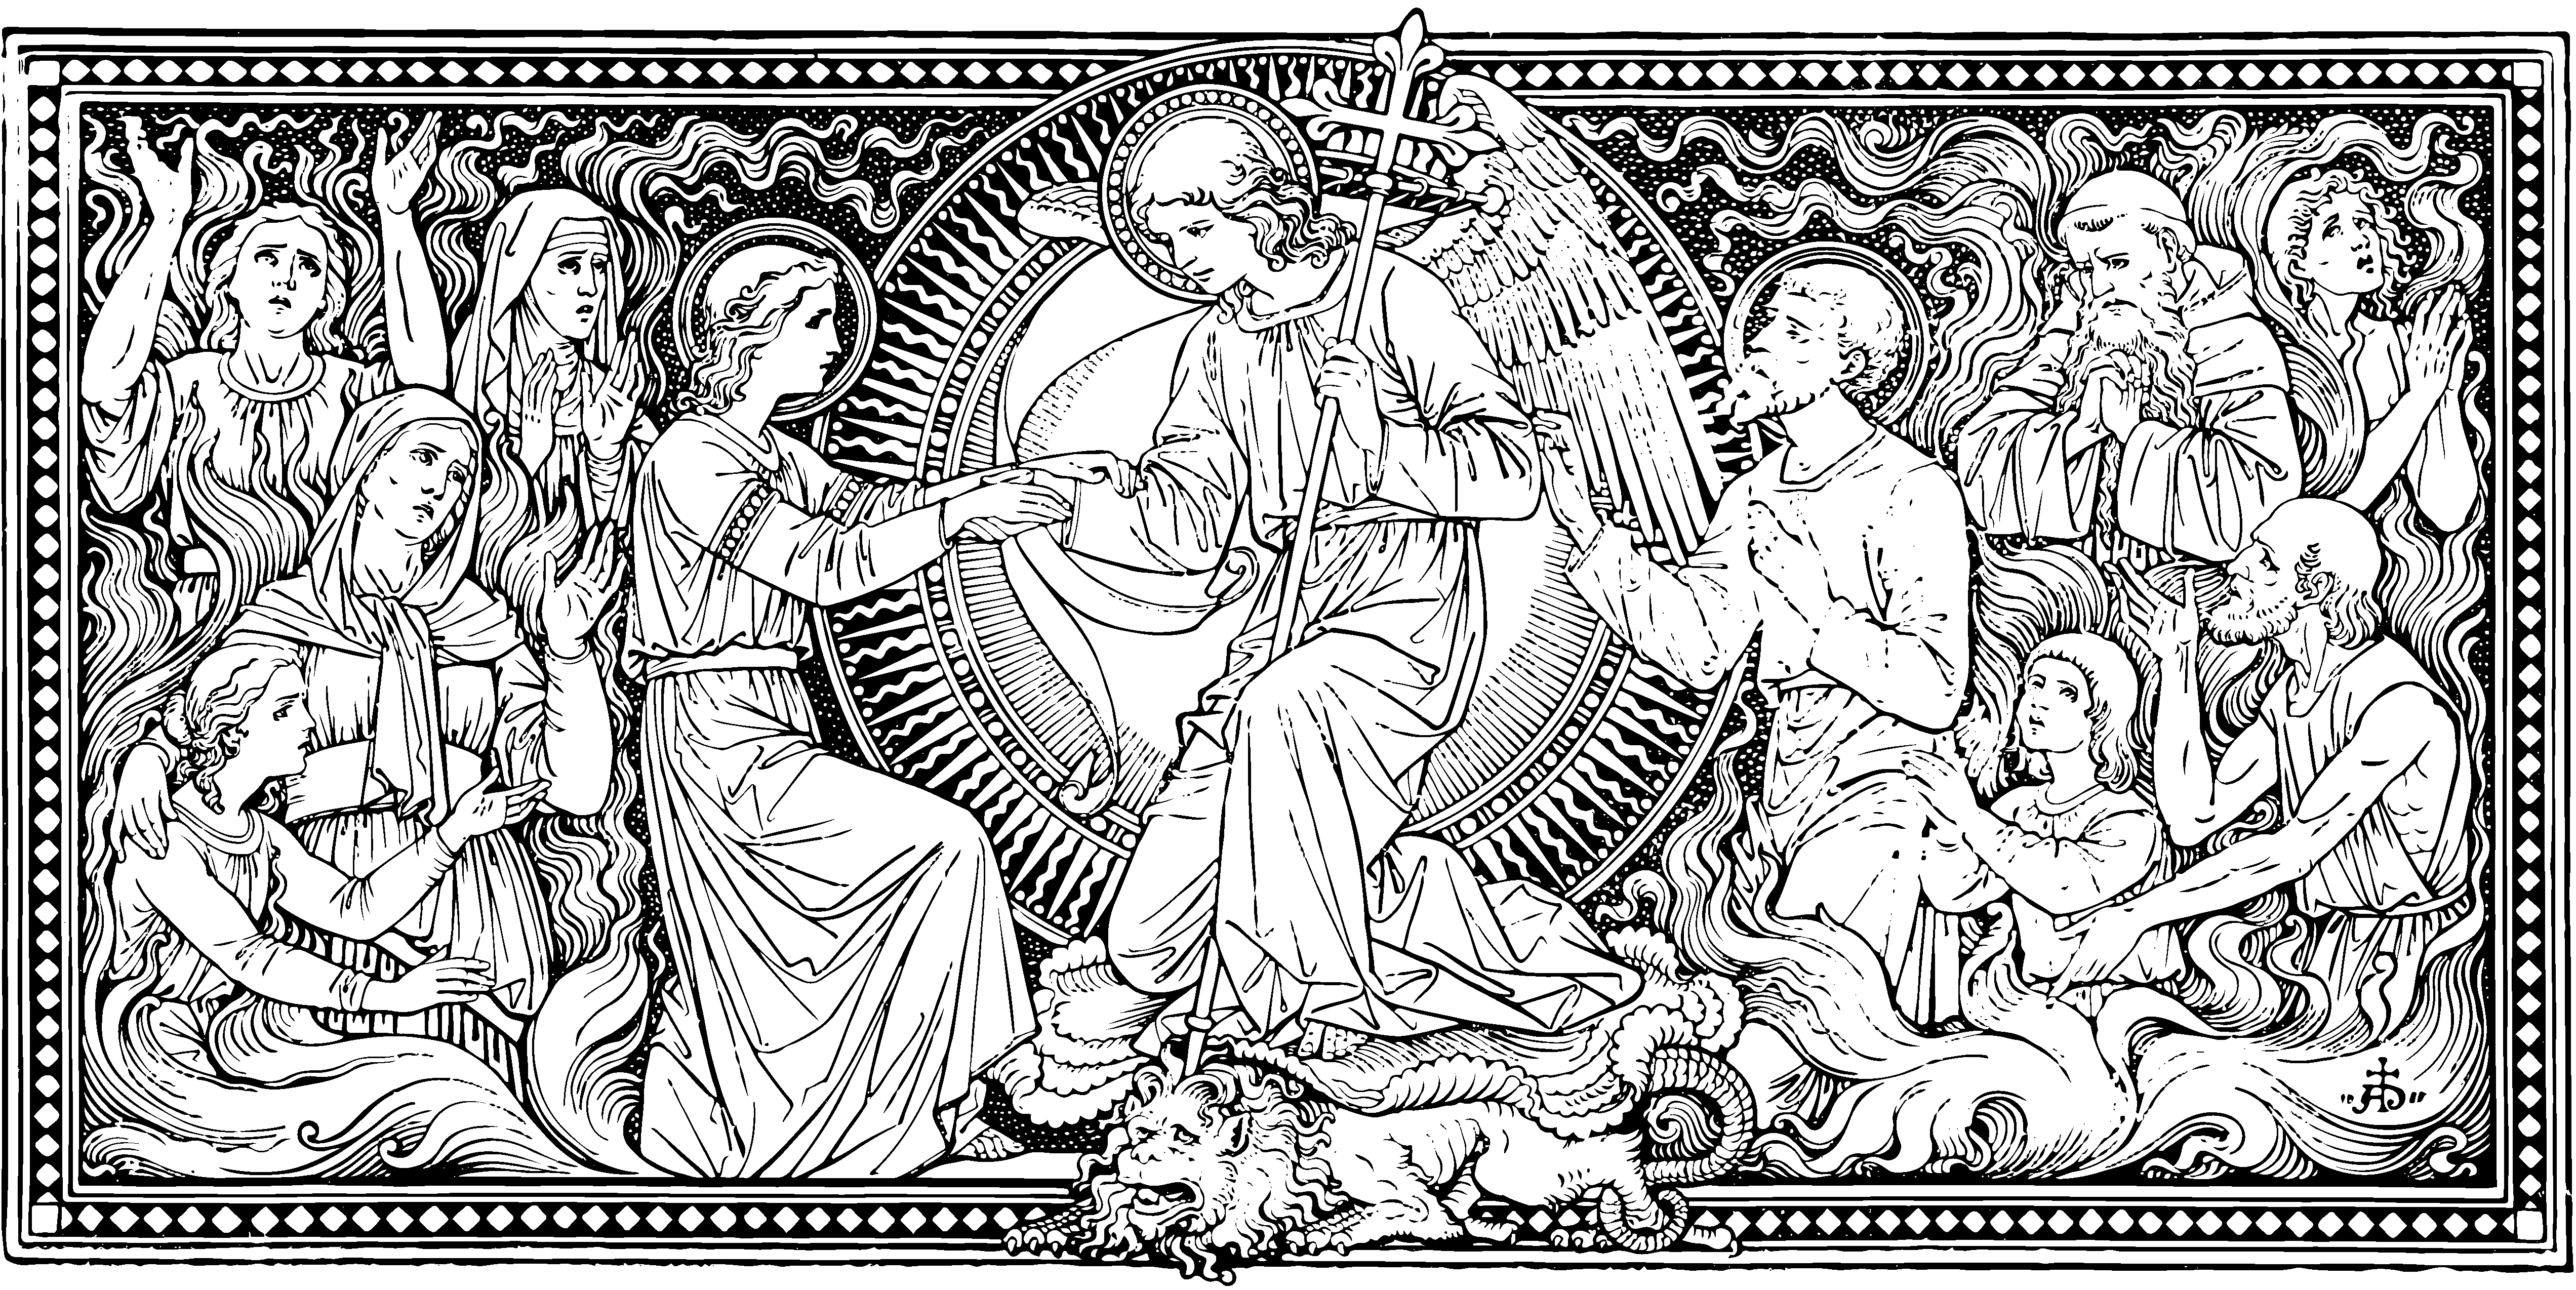
\includegraphics[width=\textwidth]{purgatory.png}\par}
\newpage
\nocturnumtitulum{Psaumes supplémentaires}
\setheaders{}{}

\rubric{Chantés à la fin des Vêpres et des Laudes, selon les rubriques antérieures aux réformes de 1960, sauf le jour de la Commémoraison de tous les fidèles défunts, les jours suivant la mort du défunt, et les autres jours où l'office était chanté selon le rite double. Aujourd'hui, l'office est toujours chanté selon le rite double, et ces psaumes sont ordinairement omis.}

\label{ps129}
\smalltitle{Psaume 129}
\smallscore[n]{EP2}
\psalmtext{129_id}
\vspace{-0.5\baselineskip}
\begin{flushright}Seigneur, donne-leur le repos éternel,~\psstar{}\\et fais luire pour eux la lumière sans déclin.\end{flushright}
\newpage
\vspace*{-2\baselineskip}
\label{ps145}
\smalltitle{Psaume 145}
\smallscore[n]{EP1}
\psalmtext{145_id}
\vspace{-0.5\baselineskip}
\begin{flushright}Seigneur, donne-leur le repos éternel,~\psstar{}\\et fais luire pour eux la lumière sans déclin.\end{flushright}



\end{document} 
